%%%%%%%%%%%%%%%%%%%%%%%%%%%%%%%%%%%%%%%%%%%%%%%%%%%%%%%%%%%%%%%
%
% For more detailed article preparation guidelines, please see:
% http://f1000research.com/author-guidelines

\documentclass[10pt,a4paper,twocolumn]{article}
\usepackage{f1000_styles}
\usepackage{hyperref}
\usepackage{longtable}
\bibliography{manuscript}

\begin{document}

%Still need to figure out how to get corresponding author on here.
\title{\textit{Associations between chlorophyll \emph{a} and various microcystin-LR
health advisory concentrations} }
\author[1]{Jeffrey W. Hollister}
\author[1]{Betty J. Kreakie}
\affil[1]{US Environmental Protection Agency, Office of Research and Development,
National Health and Environmental Effects Research Laboratory, Atlantic
Ecology Division, 27 Tarzwell Drive Narragansett, RI, 02882, USA}

\maketitle
\thispagestyle{fancy}

\begin{abstract}

Cyanobacteria harmful algal blooms (cHABs) are associated with a wide
range of adverse health effects that stem mostly from the presence of
cyanotoxins. To help protect against these impacts, several health
advisory levels have been set for some toxins. In particular, one of the
more common toxins, microcystin-LR, has several advisory levels set for
drinking water and recreational use. However, compared to other water
quality measures, field measurements of microcystin-LR are not commonly
available due to cost and advanced understanding required to interpret
results. Addressing these issues will take time and resources. Thus,
there is utility in finding indicators of microcystin-LR that are
already widely available, can be estimated quickly and in situ, and used
as a first defense against high concentrations of microcystin-LR.
Chlorophyll \emph{a} is commonly measured, can be estimated \emph{in
situ}, and has been shown to be positively associated with
microcystin-LR. In this paper, we use this association to provide
estimates of chlorophyll \emph{a} concentrations that are indicative of
a higher probability of exceeding select health advisory concentrations
for microcystin-LR. Using the 2007 National Lakes Assessment and a
conditional probability approach, we identify chlorophyll \emph{a}
concentrations that are more likely than not to be associated with an
exceedance of a microcystin-LR health advisory level. We look at the
recent US EPA health advisories for drinking water as well as the World
Health Organization levels for drinking water and recreational use and
identify a range of chlorophyll \emph{a} thresholds. A 50\% chance of
exceeding one of the specific advisory microcystin-LR concentrations of
0.3, 1, 1.6, and 2 g/L is associatied with chlorophyll \emph{a}
concentration thresholds of 24.64, 65.6, 89.71, and 94.93, respectively.
When managing for these various microcystin-LR levels, exceeding these
reported chlorophyll \emph{a} concentrations should be a trigger for
further testing and possible management action.

\end{abstract}

\textbf{Keywords: }
Harmful Algal Blooms;
Cyanotoxins;
National Lakes Assessment;
Conditional Probability Analysis;
Cyanobacteria;

\clearpage

\section{Introduction}\label{introduction}

Over the last decade, numerous events and legislative activities have
raised the public awareness of harmful algal blooms {[}1--3{]}. In
response the US Environmental Protection Agency (USEPA) has recently
released suggested microcystin-LR (one of the more common toxins)
concentrations that would trigger health advisories {[}4--6{]}.
Additionally, the World Health Organization (WHO) has proposed
microcystin advisory levels for drinking water and a range of
recreational risk levels {[}7,8{]}. While these levels and associated
advisories are likely to help mitigate the impacts from harmful algal
blooms, they are not without complications.

One of these complications is that they rely on available measurements
of microcystin-LR. While laboratory testing (e.g., chromatography)
remains the gold standard for quantifying microcystin-LR concentrations
in water samples, several field test kits have been developed. Even
though field tests provide a much needed means for rapid assessment,
they are not yet widely used and are moderately expensive (approximately
\$150-\$200 depending on specific kit) with a limited shelf life
(typically one year) {[}9,10{]}. Additionally, each technique requires
nuanced understanding of the detection method (e.g., limit of detection,
specific microcystin variants being measured, and sampling protocol).

Fortunately, microcystin-LR has been shown to be associated with several
other, more commonly measured and well understood components of water
quality that are readily assessed in the field. For instance, there are
small or hand held fluorometers that measure chlorohpyll \emph{a}.
Additionally, chlorophyll \emph{a} is a very commonly measured component
of water quality that is also known to be positively associated with
microsystin-LR concentrations {[}11,12{]}. Yuan et. al {[}12{]} explore
these associations in detail and control for other related variables. In
their analysis they find that total nitrogen and chlorophyll \emph{a}
show the strongest association with microcystin. Furthermore, they
identify chlorophyll\emph{a} and total nitrogen concentrations that are
associated with exceeding 1 \(\mu\)g/L of microcystin. Given these
facts, it should be possible to identify chlorophyll \emph{a}
concentrations that would be associated with the new USEPA
microcystin-LR health advisory levels for drinking water. Identifying
these associations would provide another tool for water resource
managers to help manage the threat to public health posed by cHABs and
would be especially useful in the absence of measured microcystin-LR
concentrations.

In this paper we build on past efforts and utilize the National Lakes
Assessment (NLA) data and identify chlorophyll \emph{a} concentrations
that are associated with higher probabilities of exceeding several
microcystin-LR health advisory concentrations {[}6,8,13{]}. We add to
past studies by exploring associations with newly announced advisory
levels and by also applying a different method, conditional probability
analysis. Utilizing different methods strengthens the evidence for
suggested chlorophyll \emph{a} levels that are associated with increased
risk of exceeding the health advisory levels as those levels are not
predicated on a single analytical method. So that others may repeat or
adjust this analysis, the data, code, and this manuscript are freely
available via
\href{https://github.com/USAPE/microcystinchla}{\url{https://github.com/USEPA/microcystinchla}}.

\section{Methods}\label{methods}

\subsection{Data}\label{data}

We used the 2007 NLA chlorophyll \emph{a} and microcystin-LR
concentration data {[}13{]}. These data represent a snapshot of water
quality from the summer of 2007 for the conterminous United States and
were collected as part of an ongoing probabilistic monitoring program
{[}13{]}. Data on chlorophyll \emph{a} and microcystin-LR concentrations
are available for 1028 lakes. These data are available for download from
the
\href{http://www.epa.gov/national-aquatic-resource-surveys/data-national-aquatic-resource-surveys}{National
Lake Assessment Data Site}

\subsection{Analytical Methods}\label{analytical-methods}

We used a conditional probability analysis (CPA) approach to explore
associations between chlorophyll \emph{a} concentrations and World
Health Organization (WHO) and USEPA microcystin-LR health advisory
levels {[}14{]}. Many health advisory levels have been suggested (Table
\ref{tab:microcystin_levels}), but lakes with higher microcystin-LR
concentrations in the NLA were rare. Only 1.16\% of lakes sampled had a
concentration greater than 10 \(\mu\)g/L. Thus, for this analysis we
focused on the microcystin concentrations that are better represented in
the NLA data. These were the USEPA children's drinking water advisory
level of 0.3 \(\mu\)g/L (USEPA Child), the WHO drinking water advisory
level of 1 \(\mu\)g/L (WHO Drinking), the USEPA adult drinking water
advisory level of 1.6 \(\mu\)g/L (USEPA Adult), and the WHO
recreational, low probability of effect advisory level of 2 \(\mu\)g/L
(WHO Recreational) {[}6--8{]}.

Conditional probability analysis provides information about the
probability of observing one event given another event has also occured.
For this analysis, we used CPA to examine how the conditional
probability of exceeding one of the health advisories changes as
chlorophyll \emph{a} increases in a lake. We expect to find higher
chlorohpyll \emph{a} concentrations to be associated with higher
probabilities of exceeding the microcystin-LR health advisory levels. We
also calculated bootstrapped 95\% confidence intervals (CI) using 1000
bootstrapped samples. Thus, to identify chlorophyll \emph{a}
concentrations of concern we identfiy the value of the upper 95\% CI
across a range of conditional probabilities of exceeding each health
advisory level. Using the upper confidence limit to identify a threshold
is justified as it ensures that a given threshold is unlikely to miss a
microcystin exceedance.

As both microcystin-LR and chlorophyll \emph{a} values were highely
skewed right, a log base 10 transformation was used. Additional details
of the specific implementation are available at
\url{https://github.com/USEPA/microcystinchla}. A more detailed
discussion of CPA is beyond the scope of this paper, but see Paul et al.
{[}15{]} and Hollister et al. {[}16{]} for greater detail. Lastly, all
analyses were conducted using R version 3.2.2 and code and data from
this analysis are freely available as an R package at
\href{https://github.com/USAPE/microcystinchla}{\url{https://github.com/USEPA/microcystinchla}}.

Lastly, we assess the ability of these chlorophyll \emph{a} thresholds
to predict microcystin exceedance. We use error matrices and calculate
total accuracy as well as the proportion of false negatives. Total
accuracy is the total number of correct predictions divided by total
observations. The proportion of false negatives is the total number of
lakes that were predicted to not exceed the microcystin guidelines but
actually did, divided by the total number of observations.

\section{Results}\label{results}

In the 2007 NLA, microcystin-LR concentrations ranged from 0.05 to 225
\(\mu\)g/L. Microcystin-LR concentrations of 0.05 \(\mu\)g/L represent
the detection limits. Any value greater than that indicates the presence
of microcystin-LR. Of those lakes with microcystin, the median
concentration was 0.51\(\mu\)g/L and the mean was 3.17\(\mu\)g/L. Of all
lakes sampled, 21\% of lakes exceeded the USEPA Child level, 8.8\% of
lakes exceeded the USEPA Adult level, 11.7\% of lakes exceeded the WHO
Drinking level, and 7.3\% of lakes exceeded the WHO Recreational level.
For chlorophyll \emph{a}, the range was 0.07 to 936 \(\mu\)g/L. All
lakes had reported chlorophyll \emph{a} concentrations that exceeded
detection limits. The median concentration was 7.79 \(\mu\)g/L and the
mean was 29.63 \(\mu\)g/L. The associations between chlorophyll \emph{a}
and the upper confidence interval across a range of conditional
probability values are shown in Table \ref{tab:mc_chla_table}. Specific
chlorophyll \emph{a} concentrations that are associated with greater
than even odds of exceeding the advisory levels were 23.36, 62.64,
83.52, and 103.9\(\mu\)g/L for 0.3, 1.0, 1.6, and 2.0 \(\mu\)g/L
advisory levels, respectively (Table \ref{tab:mc_chla_table} \& Figure
\ref{fig:multi_cp_plot}).

\begin{figure}
\centering
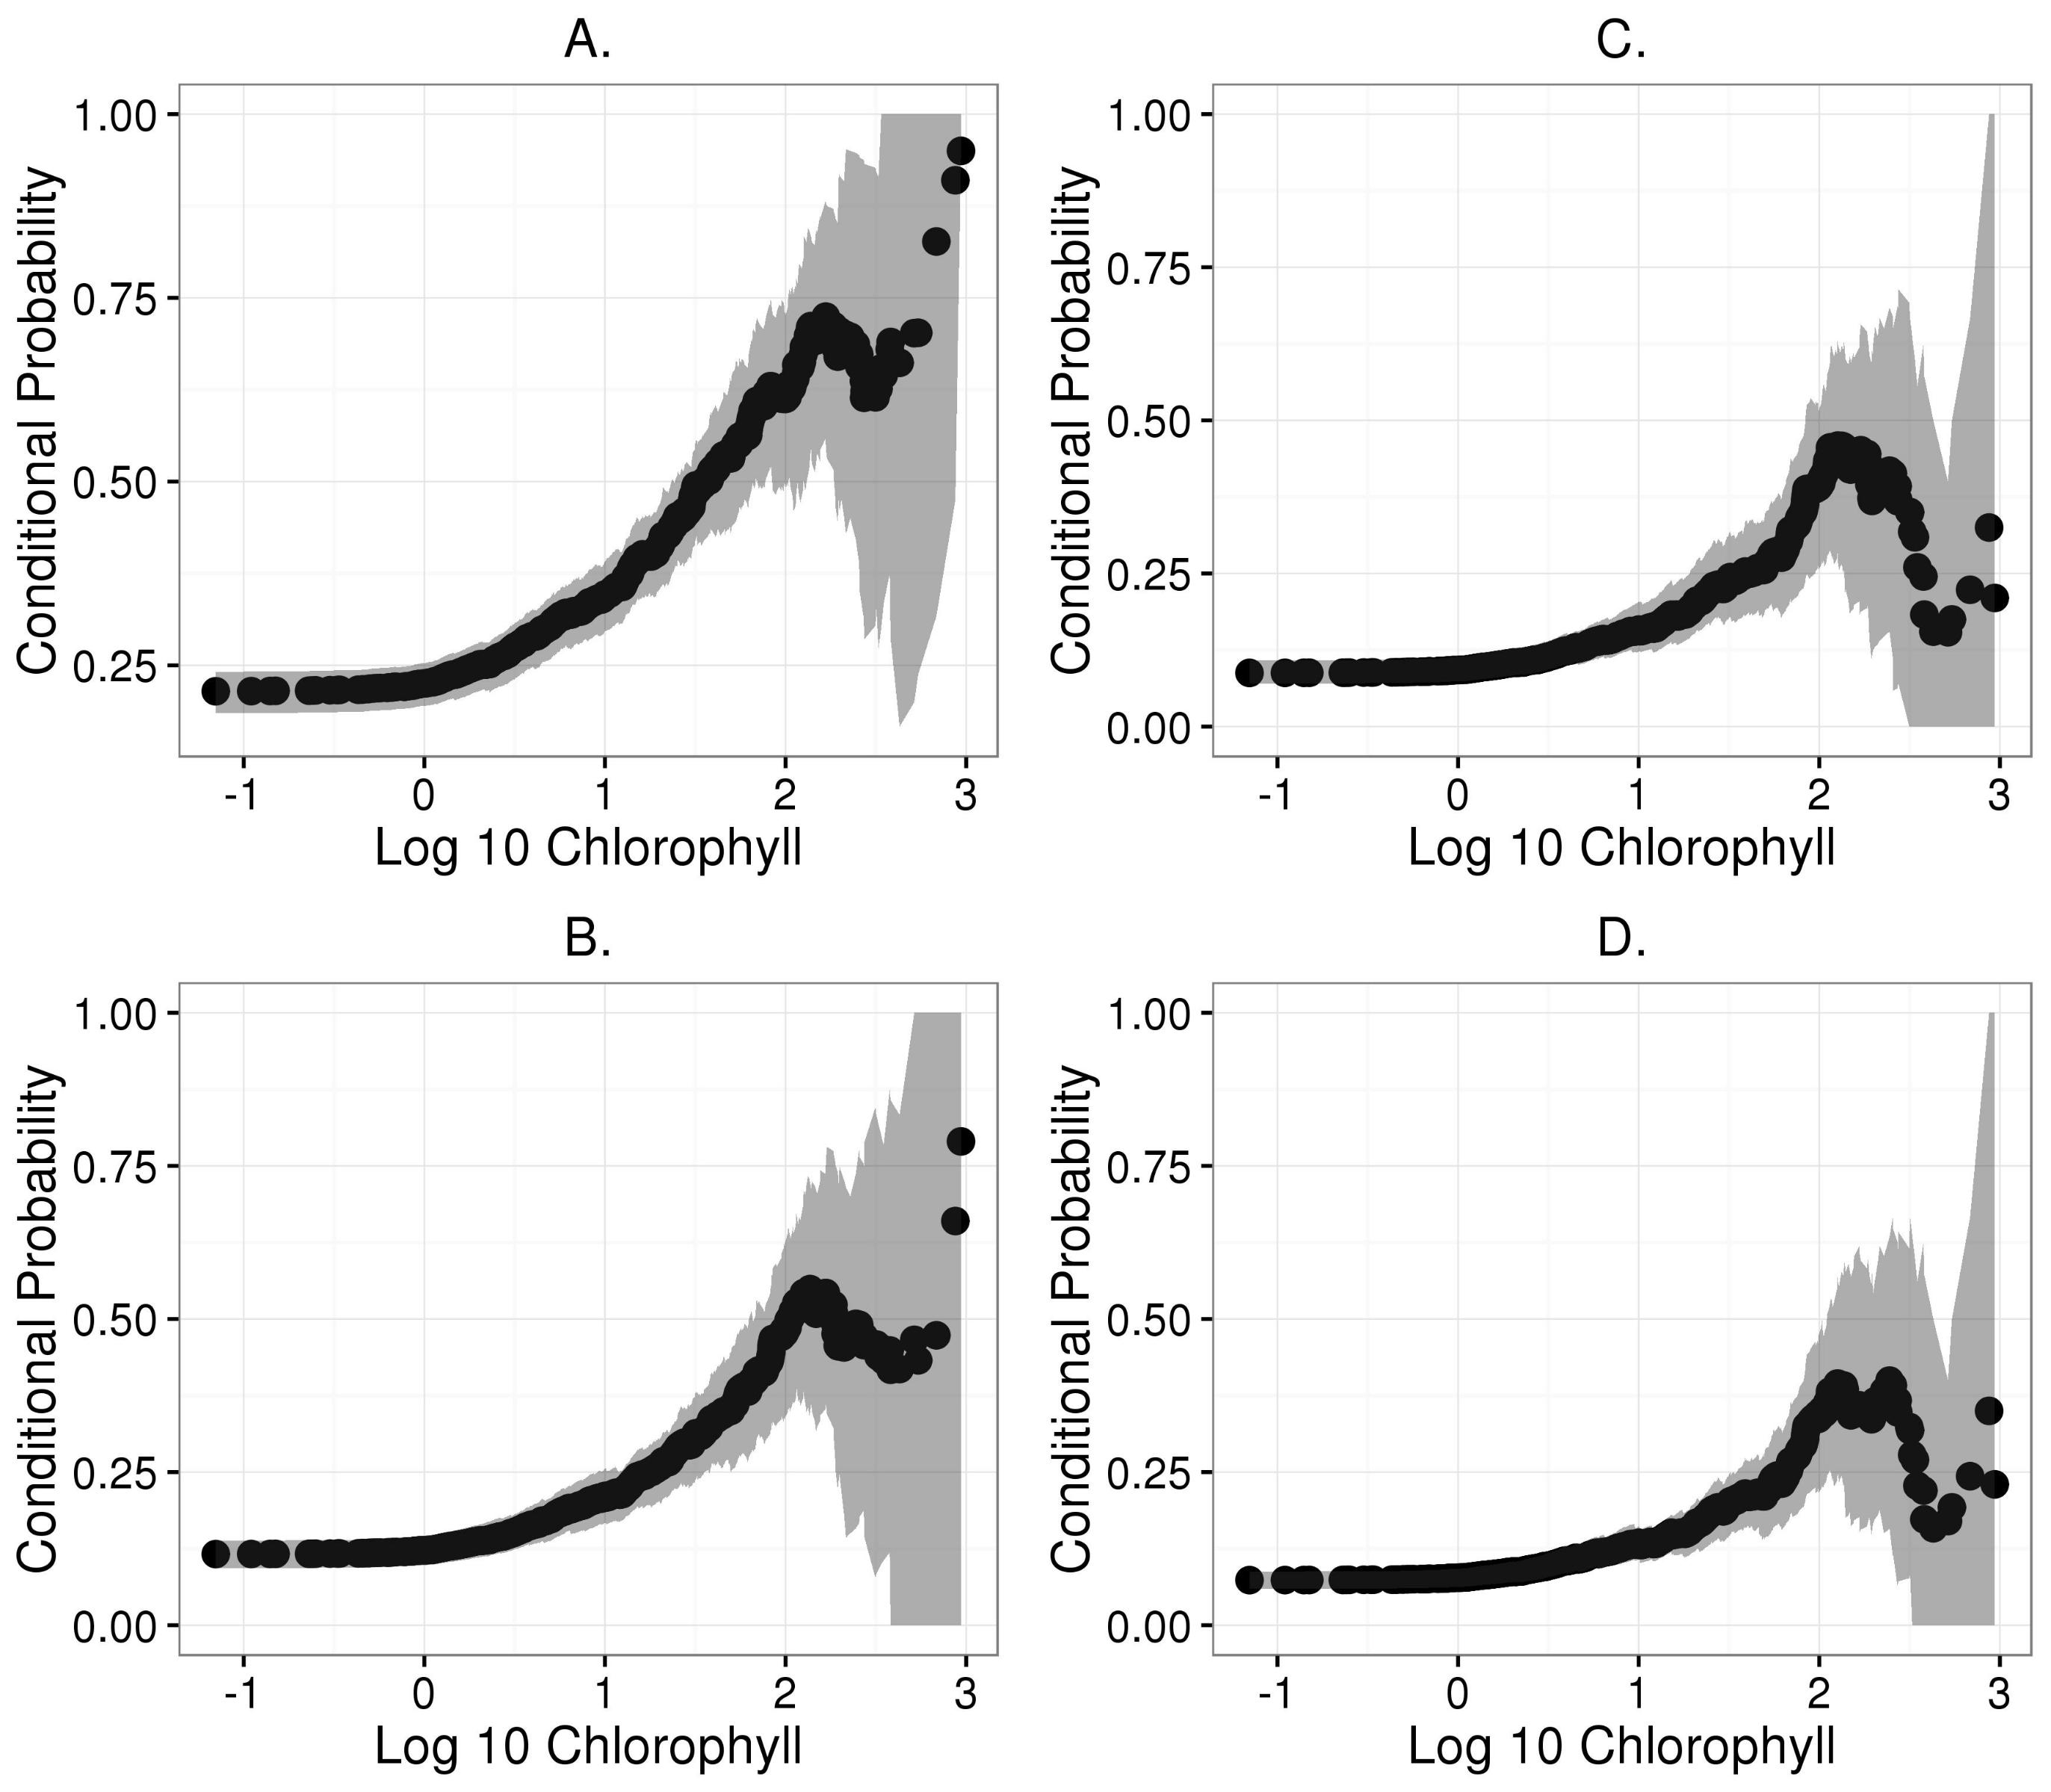
\includegraphics[width=0.4\textwidth]{hollister_microcystin_fig1.jpg}
\caption{\label{fig:multi_cp_plot}Conditional probability plots showing association between the probability of exceeding various microcystin-LR (MLR) health advisory Levels. A.) Plot for USEPA Child (0.3 $\mu$g/L). B.) Plot for WHO Drinking (1 $\mu$g/L). C.) Plot for USEPA Adult (1.6 $\mu$g/L). D.) Plot for WHO Recreational (2 $\mu$g/L).  }
\end{figure}

The chlorophyll \emph{a} cutoffs may be used to predict whether or not a
lake exceeds the microcystin-LR health advisories. Doing so allows us to
compare the accuracy of the prediction as well as evaluate false
negatives. Total accuracy of the four cutoffs predicting microcystin-LR
exceedances were 75\% for the USEPA children's advisory, 86\% for the
WHO drinking water advisory, 89\% for the USEPA adult advisory, and 91\%
for the WHO regreational advisory (Tables \ref{tab:child_conmat_table},
\ref{tab:who_drink_conmat_table}, \ref{tab:adult_conmat_table}, \&
\ref{tab:who_rec_conmat_table}). However, total accuracy is only one
part of the prediction performace with which we are concerned.

When using the chlorophyll \emph{a} cutoffs as an indicator of
microcystin-LR exceedances, the error that should be avoided is
predicting that no exceedance has occurred when in fact it has. In other
words, we would like to avoid Type II errors and minimize the proportion
of false negatives. For the four chlorophyll \emph{a} cut-offs we had a
proportion of false negatives of 9\%, 7\%, 6\%, and 5\% for the USEPA
children's, the WHO drinking water, the USEPA adult, and the WHO
recreational advisories, respectively. In each case we missed less than
10\% of the lakes that in fact exceeded the microcystin-LR advisory.
While this method performs well with regard to the false negative
percentage, it is possible that is a relic of the NLA dataset and
testing with additional data would allow us to confirm this result.

\section{Discussion}\label{discussion}

The association between Log10 microcystin-LR and Log10 chlorophyll
\emph{a} shows a wedge pattern (Figure \ref{fig:chla_micro_scatter}).
This indicates that, in general, higher concentrations of microcystin-LR
almost always co-occur with higher concentrations of chlorophyll
\emph{a} yet the inverse is not true. Higher chlorophyll \emph{a} is not
necessarily predictive of higher microcystin-LR concentrations; however,
chlorophyll \emph{a} may be predictive of the probability of exceeding a
certain threshold.

\begin{figure}
\centering
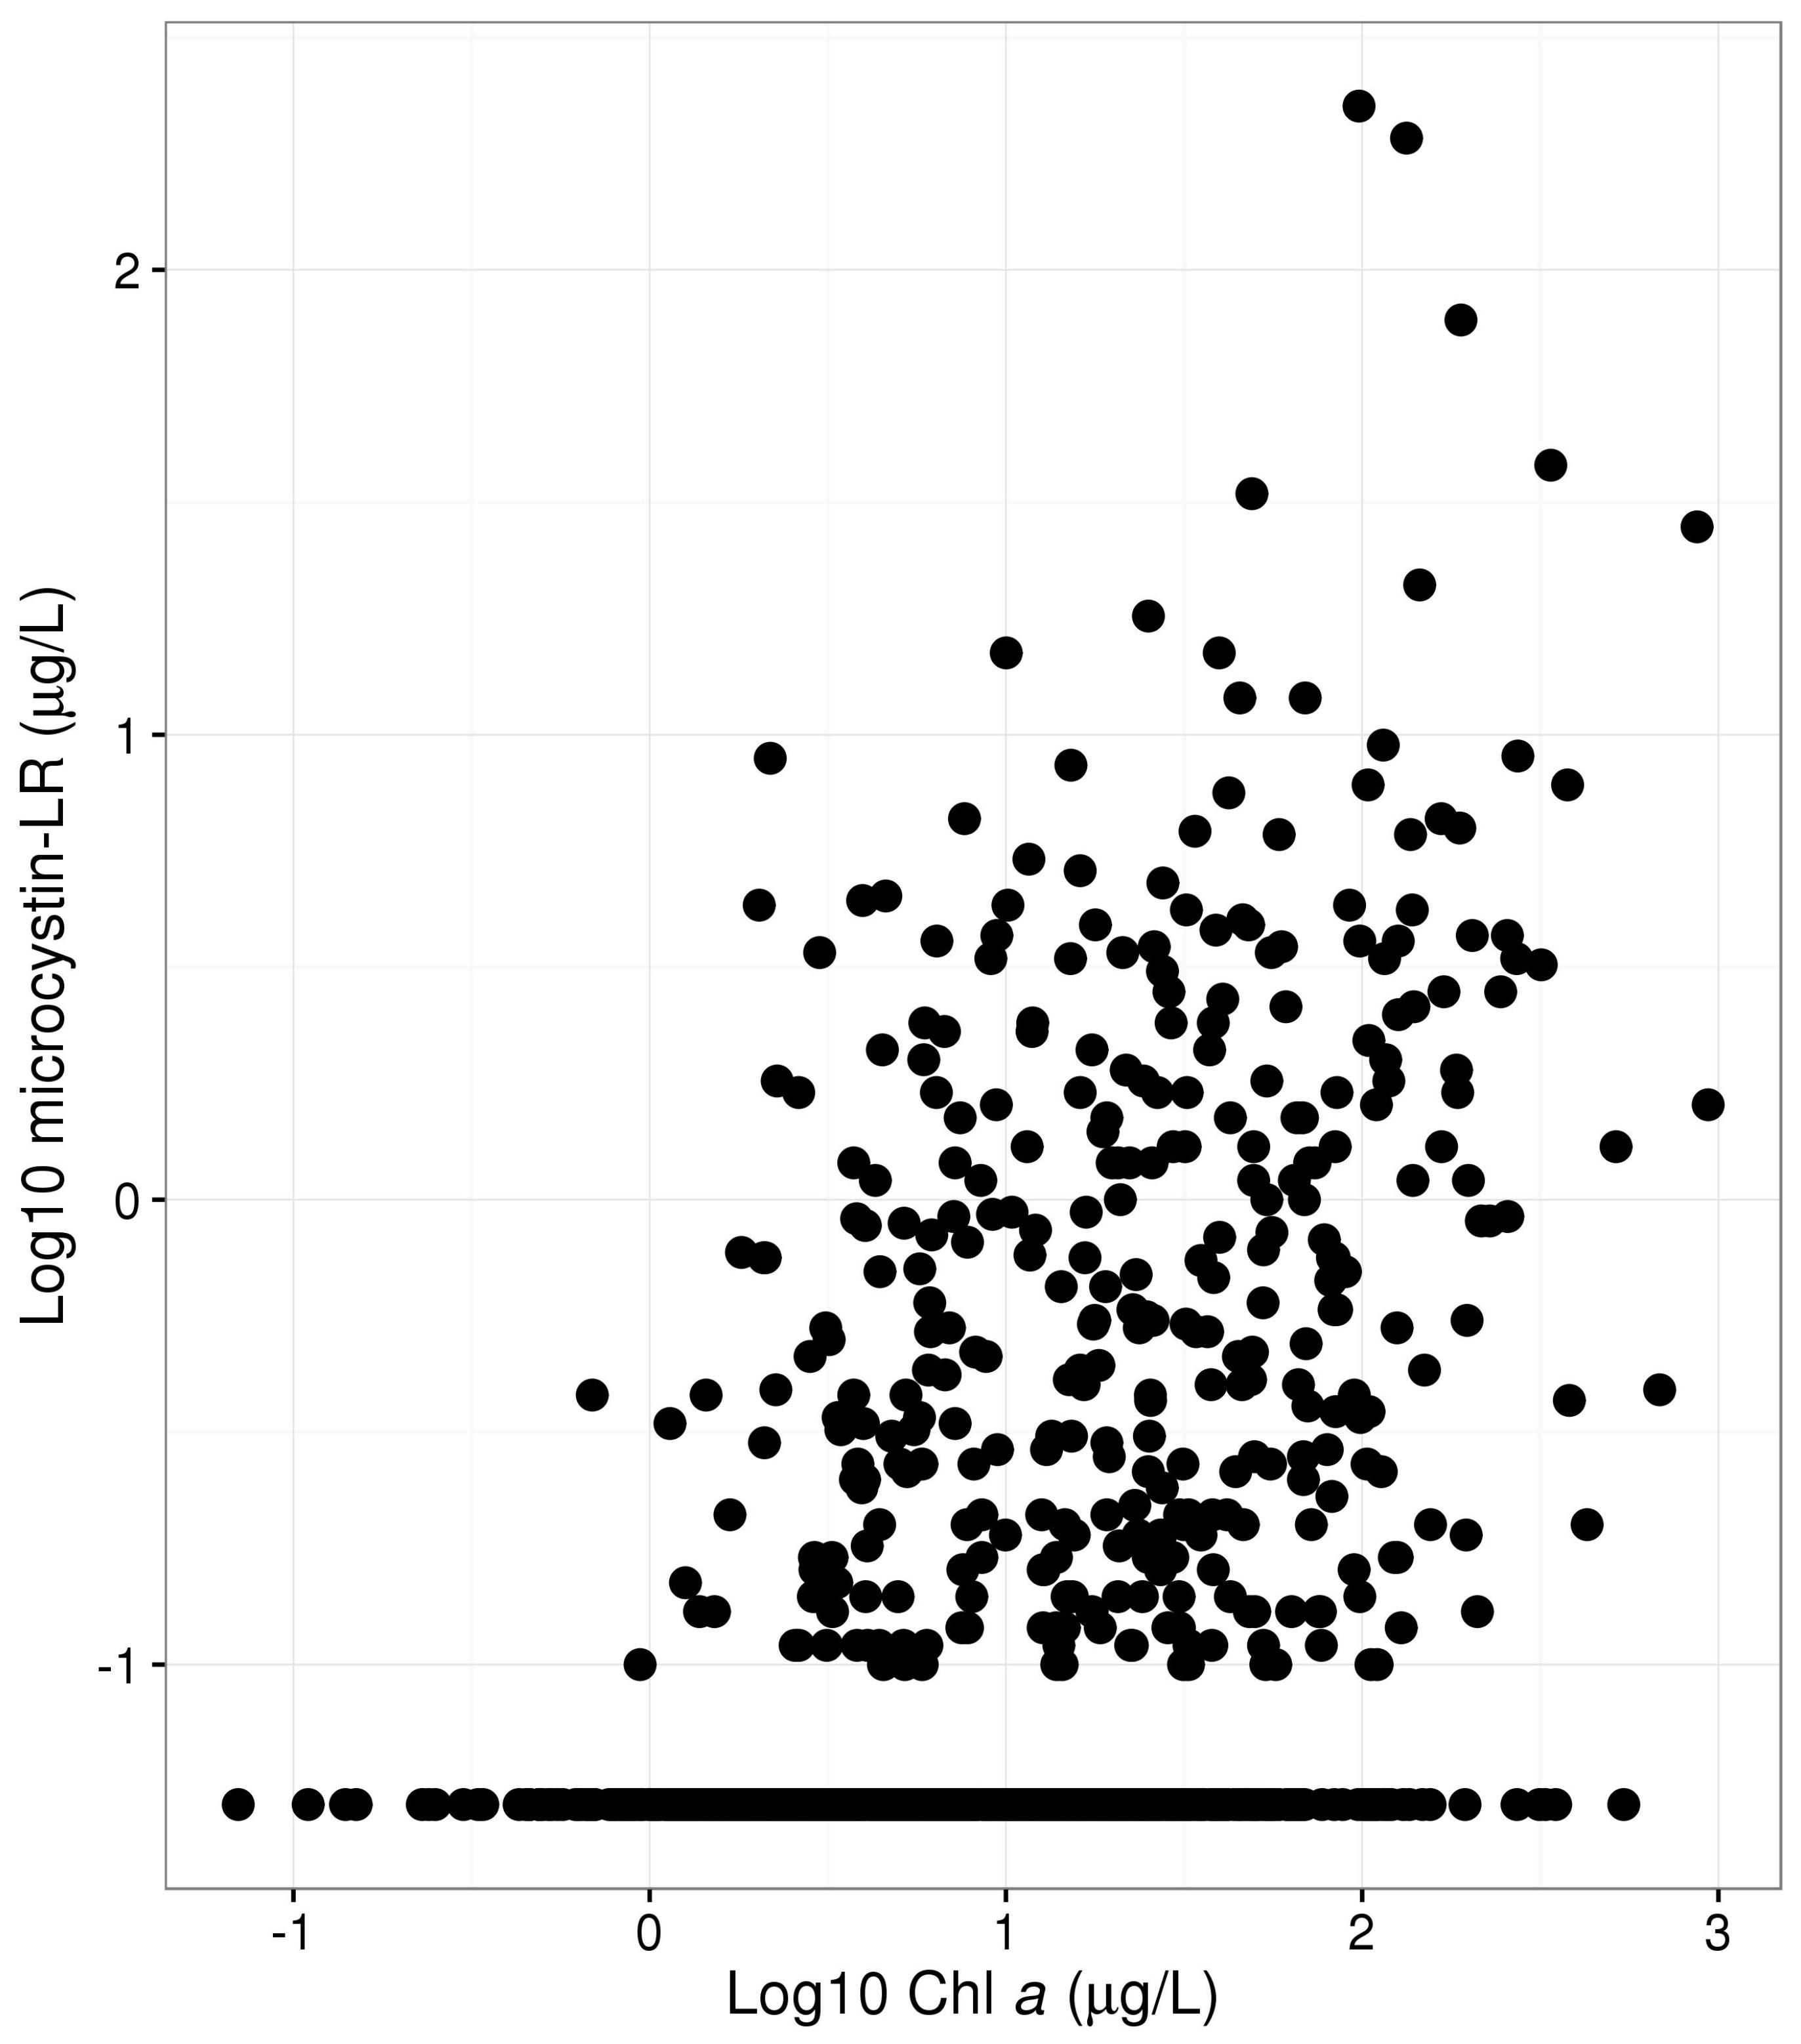
\includegraphics[width=0.4\textwidth]{hollister_microcystin_fig2.jpg}
\caption{\label{fig:chla_micro_scatter}Scatterplot showing association betweeen chlorophyll \textit{a} and microcystin-LR. }
\end{figure}

This is the case as the probability of exceeding each of the four tested
health advisory levels increases as a function of chlorophyll \emph{a}
concentration (Figure \ref{fig:multi_cp_plot}). We used this association
to identify chlorophyll \emph{a} concentrations that are associated with
a range of probabilities of exceeding a given health advisory level
(Table \ref{tab:mc_chla_table}). For the purposes of this discussion we
focus on a conditional probability of 50\% or greater (i.e., greater
than even odds to exceed a health advisory level). The 50\% conditional
probability chlorophyll \emph{a} thresholds represents 27.9\%, 12.1\%,
9\%, and 7.3\% of sample lakes for the USEPA Child, the WHO Drinking,
the USEPA Adult, and the WHO recreational levels, respecitvely.

There are numerous possible uses for the chlorophyll \emph{a} and
microcystin-LR advisory cut-off values. First, in the absence of
microcystin-LR measurements, exceedence of the chlorophyll \emph{a}
concentrations could be a trigger for further actions. Given that there
is uncertainity around these chlorophyll \emph{a} cutoffs the best case
scenario would be to monitor for chlorophyll \emph{a} and in the event
of exceeding a target concentration take water samples and have those
samples tested for microcystin-LR.

A second potential use is to identify past bloom events from historical
data. As harmful algal blooms are made up of many species and have
various mechanisms responsible for adverse impacts (e.g., toxins,
hypoxia, odors), there is no single definition of a bloom. For cHABs,
one approach has been to identify an increase over a baseline
concentration of phycocyanin {[}17{]}. This is a useful approach for
targeted studies, but phycocyanin is also not always available and
measures the predominance of cyanobacterial pigments and not toxins.
Using our chlorophyll \emph{a} cutoffs provides a value that is more
directly associated with microcystin-LR and can be used to classify
lakes, from past surveys, as having bloomed.

Lastly, using chlorophyll \emph{a} is not meant as a replacement for
testing of microcystin-LR or other toxins. It should be used when other,
direct measurements of cyanotoxins are not available. In those cases,
which are likely to be common at least in the near future, using a more
ubiquitous measurement, such as chlorophyll \emph{a} will provide a
reasonable proxy for the probability of exceeding a microcystin-LR
health advisory level and provide better protection against adverse
effects in both drinking and recreational use cases.

\section{Software and Data
Availability}\label{software-and-data-availability}

Data and Latest Source Code:
\href{https://github.com/USEPA/microcystinchla}{\url{https://github.com/USEPA/microcystinchla}}

Archived data and source code at time of publication:
\href{https://doi.org/10.5281/zenodo.45317}{\url{https://doi.org/10.5281/zenodo.45317}}

License: Creative Commons Zero 1.0:
\href{http://creativecommons.org/publicdomain/zero/1.0/}{\url{http://creativecommons.org/publicdomain/zero/1.0/}}

\section{Author Contributions}\label{author-contributions}

JH and BK conceived of and conducted the analysis. Both authors reviewed
the results and contributed to writing the manuscript.

\section{Competing Interests}\label{competing-interests}

No competing interests were disclosed.

\section{Grant Information}\label{grant-information}

The author(s) declared that no grants were involved in supporting this
work.

\section{Acknowledgements}\label{acknowledgements}

We would like to thank Anne Kuhn, Bryan Milstead, John Kiddon, Joe
LiVolsi, Tim Gleason, and Wayne Munns for constructive reviews of this
paper. This paper has not been subjected to Agency review. Therefore, it
does not necessary reflect the views of the Agency. Mention of trade
names or commercial products does not constitute endorsement or
recommendation for use. This contribution is identified by the tracking
number ORD-015143 of the Atlantic Ecology Division, Office of Research
and Development, National Health and Environmental Effects Research
Laboratory, US Environmental Protection Agency.

\onecolumn

\section{Tables}\label{tables}

\begin{table}[ht]
\caption{Various suggested microcystin-LR health advisory 
                     concentrations from the USEPA and World Health Organization.} 
\label{tab:microcystin_levels}
\begin{tabular}{lll}
  \hline
Source & Type & Concentration \\ 
  \hline
USEPA & Adult Drinking Water Advisory & 1.6 $\mu$g/L \\ 
  USEPA & Child Drinking Water Advisory & 0.3 $\mu$g/L \\ 
  WHO & Drinking Water & 1 $\mu$g/L \\ 
  WHO & Recreational: High Prob. of Effect & 20-2000 $\mu$g/L \\ 
  WHO & Recreational: Low Prob. of Effect & 2-4 $\mu$g/L \\ 
  WHO & Recreational: Moderate Prob. of Effect & 10-20 $\mu$g/L \\ 
  WHO & Recreational: Very High Prob. of Effect & >2000 $\mu$g/L \\ 
   \hline
\end{tabular}
\end{table}

\begin{table}[ht]
\caption{Chlorophyll \textit{a} concentrations that are 
                     associated with a 50% probability of exceeding a 
                     microcystin-LR health advisory concentration.} 
\label{tab:mc_chla_table}
\begin{tabular}{rrrrr}
  \hline
Cond. Probability & USEPA Child & WHO Drink & USEPA Adult & WHO Recreational \\ 
  \hline
0.10 & 0.07 & 0.07 & 0.07 & 1.65 \\ 
  0.20 & 0.07 & 4.30 & 9.52 & 20.52 \\ 
  0.30 & 2.91 & 18.72 & 25.76 & 53.64 \\ 
  0.40 & 10.88 & 38.02 & 65.60 & 82.22 \\ 
  0.50 & 23.36 & 62.64 & 83.52 & 103.90 \\ 
  0.60 & 39.80 & 94.93 & 114.62 & 155.52 \\ 
  0.70 & 65.60 & 125.40 & 273.60 & 871.20 \\ 
  0.80 & 125.28 & 314.61 & 871.20 & 871.20 \\ 
  0.90 & 197.00 & 516.00 & 871.20 & 871.20 \\ 
   \hline
\end{tabular}
\end{table}

\begin{table}[ht]
\caption{Confusion matrix comparing chlorophyll \textit{a} 
                     predicted exceedences (rows) versus real exceedances 
                     (columns) for the USEPA childrens drinking water advisory.} 
\label{tab:child_conmat_table}
\begin{tabular}{rrrr}
  \hline
 & Not Exceed & Exceed & Row Totals \\ 
  \hline
Not Exceed & 649 &  96 & 745 \\ 
  Exceed & 162 & 121 & 283 \\ 
  Column Totals & 811 & 217 & 1028 \\ 
   \hline
\end{tabular}
\end{table}

\begin{table}[ht]
\caption{Confusion matrix comparing chlorophyll \textit{a} 
                     predicted exceedences (rows) versus real exceedances 
                     (columns) for the WHO drinking water advisory.} 
\label{tab:who_drink_conmat_table}
\begin{tabular}{rrrr}
  \hline
 & Not Exceed & Exceed & Row Totals \\ 
  \hline
Not Exceed & 833 &  75 & 908 \\ 
  Exceed &  74 &  46 & 120 \\ 
  Column Totals & 907 & 121 & 1028 \\ 
   \hline
\end{tabular}
\end{table}

\begin{table}[ht]
\caption{Confusion matrix comparing chlorophyll \textit{a} 
                     predicted exceedences (rows) versus real exceedances 
                     (columns) for the USEPA adult drinking water advisory.} 
\label{tab:adult_conmat_table}
\begin{tabular}{rrrr}
  \hline
 & Not Exceed & Exceed & Row Totals \\ 
  \hline
Not Exceed & 883 &  57 & 940 \\ 
  Exceed &  54 &  34 &  88 \\ 
  Column Totals & 937 &  91 & 1028 \\ 
   \hline
\end{tabular}
\end{table}

\begin{table}[ht]
\caption{Confusion matrix comparing chlorophyll \textit{a} 
                     predicted exceedences (rows) versus real exceedances 
                     (columns) for the WHO recreational water advisory.} 
\label{tab:who_rec_conmat_table}
\begin{tabular}{rrrr}
  \hline
 & Not Exceed & Exceed & Row Totals \\ 
  \hline
Not Exceed & 908 &  50 & 958 \\ 
  Exceed &  45 &  25 &  70 \\ 
  Column Totals & 953 &  75 & 1028 \\ 
   \hline
\end{tabular}
\end{table}

\twocolumn

\section*{References}\label{references}
\addcontentsline{toc}{section}{References}

1. Jetoo S, Grover VI, Krantzberg G (2015) The toledo drinking water
advisory: Suggested application of the water safety planning approach.
Sustainability 7: 9787--9808.

2. Rinta-Kanto JM, Konopko EA, DeBruyn JM, Bourbonniere RA, Boyer GL, et
al. (2009) Lake erie microcystis: Relationship between microcystin
production, dynamics of genotypes and environmental parameters in a
large lake. Harmful Algae 8: 665--673.

3. Harmful Algal Bloom and Hypoxia Research and Control Amendments Act
(2014) Harmful Algal Bloom and Hypoxia Research and Control Amendments
Act of 2014. (S. 1254). Available:
\url{https://www.congress.gov/113/bills/s1254/BILLS-113s1254enr.pdf}.

4. McElhiney J, Lawton LA (2005) Detection of the cyanobacterial
hepatotoxins microcystins. Toxicology and Applied Pharmacology 203:
219--230.

5. Zurawell RW, Chen H, Burke JM, Prepas EE (2005) Hepatotoxic
cyanobacteria: A review of the biological importance of microcystins in
freshwater environments. Journal of Toxicology and Environmental Health,
Part B 8: 1--37.

6. USEPA (2015) Drinking water health advisory for the cyanobacterial
microcystin toxins. EPA-820-R-15100. Available:
\url{http://www2.epa.gov/sites/production/files/2015-06/documents/microcystins-report-2015.pdf}.

7. World Health Organization (2003) Cyanobacterial toxins:
Microcystin-LR in drinking-water. Background document for development of
WHO guidelines for drinking-water quality. Geneva, Switzerland. World
Health Organization, 2nd ed. Geneva.

8. Chorus EI, Bartram J (1999) Toxic cyanobacteria in water: A guide to
their public health consequences, monitoring and management. World
Health Organization.

9. James R, Gregg A, Dindal A, McKernan J (2011) Environmental
technology verification report: Abraxis microcystin test kits. Online
document. Accessed online: June 22.

10. Aranda-Rodriguez R, Jin Z, Harvie J, Cabecinha A (2015) Evaluation
of three field test kits to detect microcystins from a public health
perspective. Harmful Algae 42: 34--42.

11. Pip E, Bowman L (2014) Microcystin and algal chlorophyll in relation
to nearshore nutrient concentrations in Lake Winnipeg, Canada.
Environment and Pollution 3: p36.

12. Yuan LL, Pollard AI, Pather S, Oliver JL, D'Anglada L (2014)
Managing microcystin: Identifying national-scale thresholds for total
nitrogen and chlorophyll a. Freshwater Biology 59: 1970--1981.

13. USEPA (2009) National lakes assessment: A collaborative survey of
the nation's lakes. EPA 841-R-09-001.

14. Paul JF, Munns WR (2011) Probability surveys, conditional
probability, and ecological risk assessment. Environmental Toxicology
and Chemistry 30: 1488--1495.

15. Paul JF, McDonald ME (2005) Development of empirical, geographically
specific water quality criteria: A conditional probability analysis
approach. Journal of the American Water Resources Association 41:
1211--1223.

16. Hollister JW, Walker HA, Paul JF (2008) CProb: A computational tool
for conducting conditional probability analysis. Journal of
Environmental Quality 37: 2392--2396.

17. Miller TR, Beversdorf L, Chaston SD, McMahon KD (2013)
Spatiotemporal molecular analysis of cyanobacteria blooms reveals
microcystis-aphanizomenon interactions. PloS one 8: e74933.

\end{document}
